
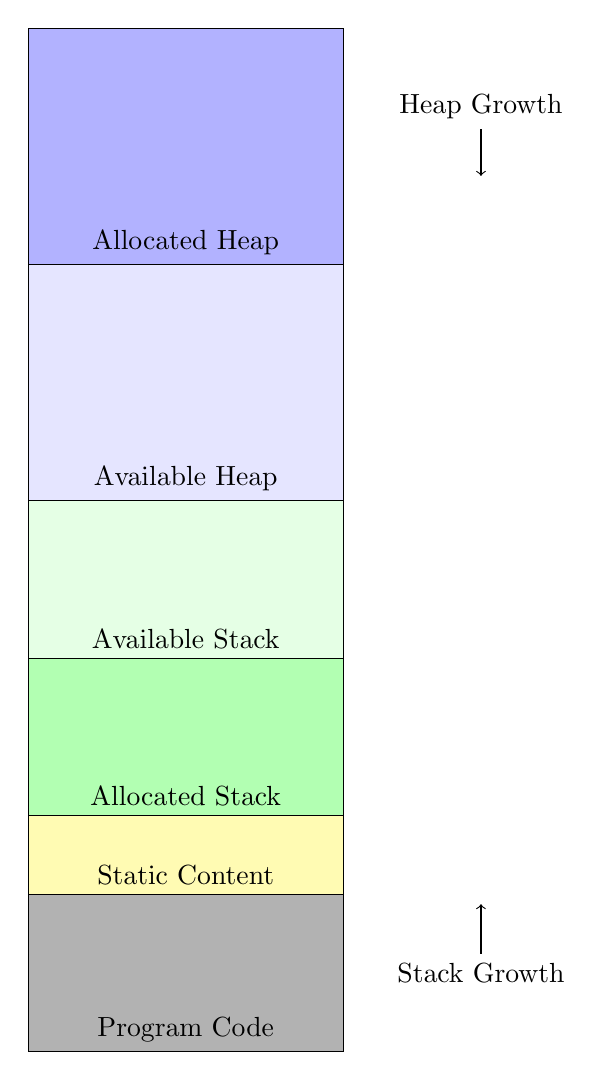
\begin{tikzpicture}[auto,scale=1.0,transform shape,every node/.style={text centered}]

%\path [top color=green!10!white, bottom color=white] (0,3) rectangle (6,5);

\path [draw,fill=black!30!white] (0,0) rectangle (4,2);
\path [draw,fill=yellow!30!white] (0,2) rectangle (4,3);
\path [draw,fill=green!30!white] (0,3) rectangle (4,5);
\path [draw,fill=green!10!white] (0,5) rectangle (4,7);
\path [draw,fill=blue!10!white] (0,7) rectangle (4,10);
\path [draw,fill=blue!30!white] (0,10) rectangle (4,13);

\node [above] (pc) at (2, 0) {Program Code};
\node [above] (static) at (2, 2) {Static Content};
\node [above] (ustack) at (2, 3) {Allocated Stack};
\node [above] (astack) at (2, 5) {Available Stack};
\node [above] (aheap) at (2, 7) {Available Heap};
\node [above] (uheap) at (2, 10) {Allocated Heap};

\node (sg) at (5.75, 1) {Stack Growth};
\node[above of=sg] (phantomsg) {~};
\draw[->] (sg) -- (phantomsg);

\node (hg) at (5.75, 12) {Heap Growth};
\node[below of=hg] (phantomhg) {~};
\draw[->] (hg) -- (phantomhg);

\end{tikzpicture}



